\chapter{Developmental stability of the \abbr{mrna}--\abbr{trna} interface}

In order to study how changes in \mrna gene expression relate to changes in
\trna gene expression, we collected tissue samples from six time points in mouse
(\mmu) development: two before birth (E15.5 and E18.5, which stands for
\num{15.5} and \num{18.5} days after gestation of the oocyte, respectively); two
shortly after birth, happening around E20 (P0.5 and P4 --- \num{0.5} and \num{4}
days after birth, respectively) and two after weaning the juvenile mice (P22 and
P29).

For each of these time points, tissue was collected from whole liver and whole
brain (homogenised) and prepared for \rnaseq and \pol3 \chipseq in order to
assay \mrna and \trna gene expression. The tissues were chosen for their
interesting shifts in physiology during development: the liver is a homogeneous
organ predominantly made up of a single cell type --- around \num{70} per cent
hepatocytes\todo{ref} --- and liver function changes fundamentally at birth;
prenatal liver serves mainly as a haematopoietic organ, whereas liver of
post-natal mice is primarily a metabolic organ.\todo{ref} Brain, by contrast, is
a highly heterogeneous organ made up of many different cell types, with dynamic
changes all through development.\todo{ref}

Each experiment was performed in two biological replicates, which were highly
correlated. \Cref{fig:trna-project-outline} summarises the experimental
procedure.\footnote{The wet-lab work of this project was performed by Bianca
Schmitt.}

\textfig[\todo{Remove background gradients from graphics}]{trna-project-outline}{body}{0.8\textwidth}
    {Sample analysis outline}
    {Samples were collected in eight distinct time points …}

In addition to the six time points described above, tissue was also collected at
two earlier stages, E9.5 and E12.5. Unfortunately, the embryo at such early
stages of development is too small to permit collecting enough tissue-specific
material. For that reason, we used the whole embryo at E9.5 and separated the
E12.5 embryo into torso and upper body. The subsequent analysis was performed on
the six later stages in liver and brain, unless noted otherwise.\todo{never
mentioned again} However, the earlier stages were able confirm the general
patterns found by analysing the remaining data.\todo{add supplementary PCA}

The results presented in this chapter are published as \citet{Schmitt:2014}.

%\section{Mouse tissue development as a model system to study mRNA and tRNA gene
%regulation}

\section{Protein-coding gene expression changes dynamically during mouse
development}

In order to investigate how protein-coding genes change expression during
development, we used the generated \rnaseq expression data, which reports counts
for each gene in each condition proportional to the expression strength times
the length of that gene.

Changes in the expression of protein-coding genes, leading to changes in
abundance of proteins, are known to drive cellular behaviour\todo{ref}. Our data
confirms that tissue development in mice is accompanied by large-scale changes
to the \mrna transcriptome. This is nicely illustrated by looking at individual
gene expression counts, plotted against their genomic location
(\cref{fig:mrna-expression-change}). For example, we can confirm the functional
relevance of apolipoprotein B (\protein{APOB}) as the primary carrier of
lipoproteins, which becomes increasingly relevant as the organ shifts to
metabolism \citep{Knott:1986}. Similarly, \mrna gene expression changes
highlight the role of α-fetoproteine (\protein{AFP}) as the fetal version of
serum albumin (\cref{fig:apob-afp}) \citep{Chen:1997}.\todo{Explain brain
examples as well?}

\textfloat{mrna-expression-change}{spill}{%
    \centering
    \begingroup
        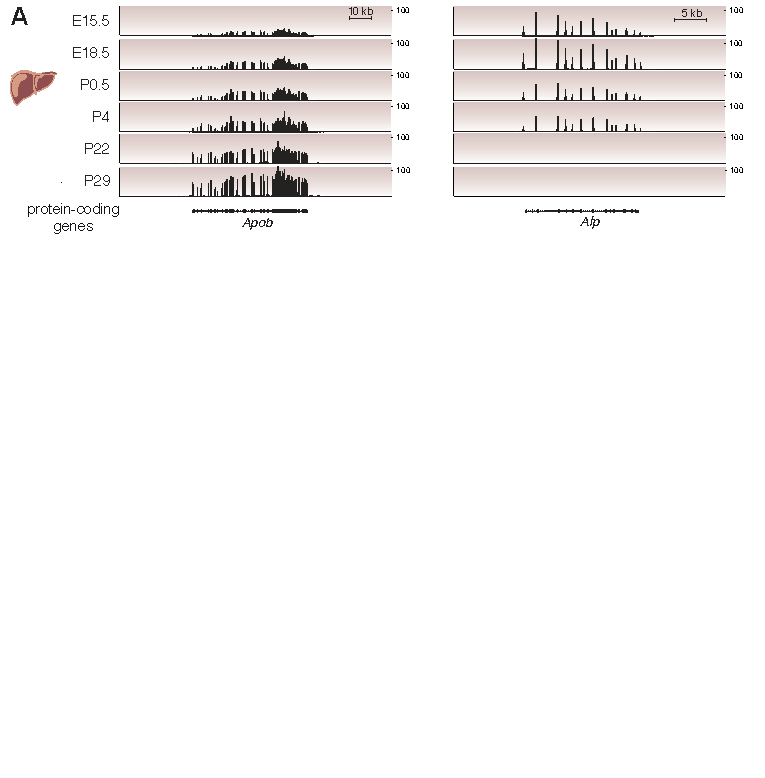
\includegraphics[width=\textwidth]{liver-mrna-expression-change}
        \subcaption{\label{fig:apob-afp}Gene expression changes of \gene{Apob} and \gene{Afp}.}
    \endgroup
    \par
    \begingroup
        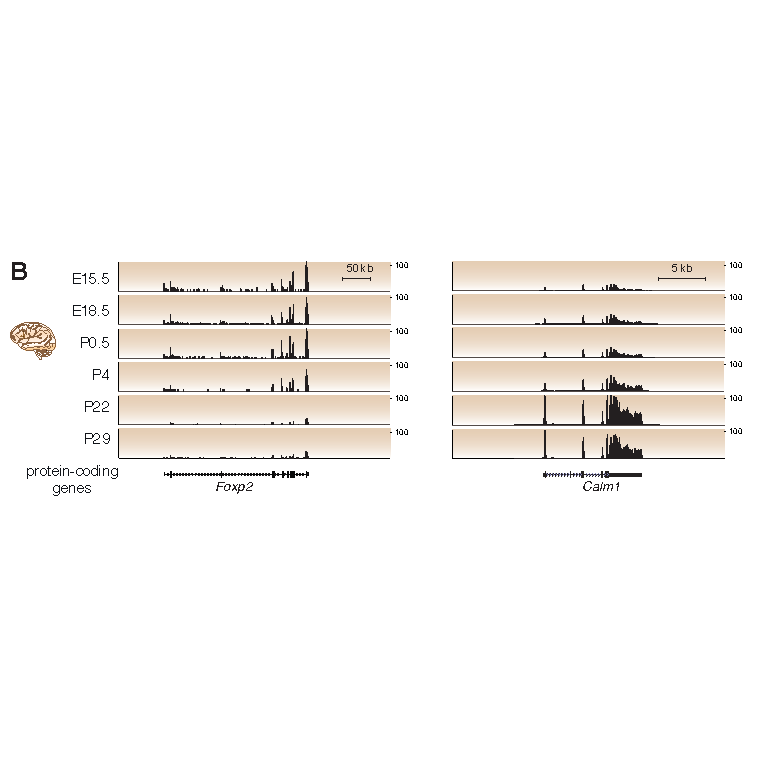
\includegraphics[width=\textwidth]{brain-mrna-expression-change}
        \subcaption{Gene expression changes of \gene{Foxp2} and \gene{Calm1}.}
    \endgroup}
    {Example of gene expression changes in development.}
    {The four genes are representative for tissue- and stage-specific genes,
    whose expression changes drive cell function. These changes can go up or
    down over the course of development, correspoding to either an up- or
    downregulation.}

For a more systematic analysis, I took the matrix of normalised count data of
all library replicates and all \mrna[s], \(m_{ij}\), for each \mrna gene \(i\)
and each library replicate \(j\), and calculated pairwise Spearman rank
correlations between all replicates,

\begin{equation}
    c_{ij} = \operatorname{cor}(m_{\dots i}, m_{\dots j}) \text{\ for all
        libraries \(i\), \(j\).}\todo{check typography}
\end{equation}

I then performed \pca on the correlation matrix, which allows to project the
variation in the data onto uncorrelated axes, so that the first axis represents
the greatest variance of the data, and the second axis represents the second
greatest variance.

The resulting \pca in \cref{fig:mrna-pca} shows that the biggest source of
variance in the correlation structure of the expression data is tissue identity,
which explains \num{97} per cent of the total variance. However, of the
remaining variance, \num{60} per cent is explained by progression of tissue
development in a way which nicely mirrors biology: the plot’s \(y\) axis shows
the linear progression of development from early stages at the bottom to late
stages at the top.

Next, I used \name{DESeq2} \citep{Love:2014} to call differentially expressed
genes between stages and tissues. Genes are counted as differentially expressed
here if their Benjamini–Hochberg \fdr-corrected \(p\)-value is below
\num{0.001}. The number of differentially expressed genes between all pairwise
developmental stages unsurprisingly shows that more distinct developmental
stages having higher numbers of differentially expressed genes
(\cref{fig:mrna-de-matrix}). Furthermore, there is a clear gap between pre- and
post-weaning stages, with a large jump in the number of differentially expressed
genes across the weaning boundary, in both liver and brain.

\textfigtwo{mrna-pca}
    {\pca of \mrna gene expression per developmental stage.}
    {Rotations \num{1} and \num{2} of the correlation matrix of
    protein-coding gene expression in each developmental stage. The percentage
    on the axes shows the amount of variance explained by each rotation.}
    {mrna-de-matrix}
    {Number of differentially expressed \mrna genes between stages:}
    {Each off-diagonal square shows the number of differentially
    expressed genes (at a significance threshold of \(p<0.01\)) between
    the two indicated developmental stages.}

These patterns are noteworthy because they recapitulate tissue identity and
linear progression through the stages of tissue development. But they are not
particularly surprising: after all, cell function is dictated by specific
protein abundance and thus protein-coding gene transcription --- the patterns of
gene expression similarity shown in the \pca and in the number of differentially
expressed genes therefore recapitulate the expected changes in cell function
between tissues, and over the course of development.

\section{Dynamic changes of \trna gene expression during mouse development}

I treated \trna gene expression count data in the same way as the \mrna gene
expression data, with one exceptions: as described in \cref{sec:chip}, I
filtered unexpressed \trna genes using a fixed threshold. The following analysis
is thus using only the \num{311} expressed out of \num{433} total genes
(\num{72} per cent).

Unlike protein-coding genes, \trna genes are not directly implicated in changes
of cellular function. We therefore did not expect many changes of the levels of
\trna gene expression over the course of development, and we do in fact observe
that many \trna gene expression levels remain stable (\cref{fig:trna-counts}).
Nevertheless, we also observe that around \num{50} per cent of all \trna genes
\emph{are} differentially expressed. \Cref{fig:liver-trna-expression-change}
shows a genomic location containing \trna genes which display these different
dynamics.

\textfigtwo{trna-counts}
    {Overview over \trna gene expression change.}
    {Bar plots show different types of \trna gene expression dynamics: \trna
    genes without change in their expression levels, \trna genes with changes to
    their expression levels, which are nevertheless expressed in all stages of
    development across both tissues; and \trna genes which are only expressed in
    a subset of all conditions.}
    {liver-trna-expression-change}
    {Example of dynamically changing \trna genes.}
    {Genomic region showing different types of \trna gene expression behaviour;
    the label colours on the x axis corresponds to the colours in
    \cref{fig:trna-counts}}

Surprisingly, the \trna gene expression differences follow similar patterns to
those observed in \mrna genes when plotting the first two principal components
of the \pca of the rank correlated replicates (\cref{fig:trna-pca}). The
observed patterns are incompatible with mere \emph{random} expression changes
(which would result in an unordered cloud of points). Something must account for
these concerted changes in \trna gene expression.

\textfig{trna-pca}{body}{0.5\textwidth}
    {\pca of \trna gene expression per developmental stage.}
    {Rotations \num{1} and \num{2} of the correlation matrix of
    \trna gene expression in each developmental stage. The percentage on the
    axes shows the amount of variance explained by each rotation.}

In the case of the protein-coding genes, we can explain the nonrandom changes in
gene expression by known gene regulatory mechanisms, which control the
transcriptome of each cell and developmental stage. The fact that \trna gene
expression changes across development exhibit the same patterns as \mrna gene
expression changes suggests that \trna gene expression is subject to similar
regulatory constraints. We therefore attempted to explain \emph{why} \trna gene
expression requires changing in a regulated manner, and \emph{how} this \trna
gene regulation is carried out by the cell.

Our first suspicion was that changes in \mrna gene expression might lead to
changes in codon demand, since different protein-coding genes are made up from
different codons. The change in codon demand in turn could lead to a change in
anticodon supply in the form of differential \trna gene expression. This would
meet the need for efficient translation: mismatching codon and anticodon pools
would either lead to a wasteful over-production of \trna[s] of a given
anticodon, or to a bottleneck in such an anticodon supply, causing efficiency
loss in translation. Both scenarios present a non-optimal scenario for the
fitness of the cell and should reasonably be selected against.

We therefore went on to quantify the codon pool corresponding to each given
transcriptome\footnote{I shall refrain from using the term “codome” to refer to
the -ome of codons}, as well as the pool of available \trna genes, grouped by
their anticodon isoacceptor identity.

\section{Every mouse \mrna transcriptome encodes the same distribution of
triplet codons and amino acids}

The codon pool of a given \mrna transcript is given by the distribution of
triplet codons in its sequence. There are 64 possible triplet codons, of which
61 encode 20 different amino acids, and three encode the stop codon, marking the
end of translation.\footnote{My analysis ignores selenocysteine, which is a
\num{21}st possible amino acid, and which can be encoded by the stop codons
\codon{UGA} under rare circumstances.} Using this information and the transcript
abundance, quantified by our \rnaseq data, I calculated the abundance of each
triplet codon as well as each amino acid in the transcriptome of each
developmental stage. I then compared these across stages to find out how they
varied.

First, for every gene, the number of occurrences of each codon in the longest
annotated transcript (the “canonical” transcript) was determined and this value
was multiplied by the gene’s expression (normalised for transcript length).
Next, the overall usage of each codon was obtained by summing these values
across all genes. Relative codon and usage (excluding selenocysteine) were
calculated using

\begin{equation}
    x_{ij}^* = x_{ij}\left(\sum_{k=1}^n x_{kj}\right)^{-1},
\end{equation}

where \(x_{ij}\) is the triplet codon usage for triplet codon \(i\) in stage
\(j\), and \(x_{ij}^*\) is the relative usage.

We find that on the transcriptome level, codon abundance is highly stable across
development in both tissues (Spearman’s \(\rho > 0.97\)) ---
\cref{fig:codon-anticodon-abundance} top left shows this by way of example using
the codons for arginine in the different stages in liver.

Given this stability, we wondered how much variation should be expected, by
simulating random transcriptomes, and computing their codon usage.

I used our library-size normalised \rnaseq data to simulate background
distributions in liver and brain for each specific developmental stage. I
randomly rearranged the expression values across genes for the expressed
(“\textsc{expr}”) and all genomically annotated (“\textsc{all}”) protein-coding
genes. For each developmental stage, I created \num{100} such random background
distributions. I then calculated the triplet codon usage for the rearranged
protein-coding \rna expression distributions.

\Cref{fig:codon-anticodon-abundance} top middle and right shows that even for
simulated transcriptomes the codon usage remains unchanged. In fact, both
observed and simulated transcriptomes seem to simply reflect the codon abundance
found in the coding part of the genome, regardless of the sometimes strong
variations in gene expression between different transcriptomes.

\textfig{codon-anticodon-abundance}{spill}{0.8\textwidth}
    {Codon and anticodon abundance across stages of development.}
    {The figure consists of three panels (right, middle, left) with three
    subfigures (top, centre, bottom) each. The left panel shows observed data
    for each of the developmental stages in liver (brain data is comparable).
    The middle and right panels show simulated data from randomised
    transcriptomes. The middle panel used only expressed genes of each
    respective stage in the simulated data, whereas the right panel uses all
    genes, also unexpressed ones). The top figures of each panel show relative
    \mrna transcript triplet codon usage, using the representative example of
    arginine. The centre figures show the relative \trna anticodon abundance of
    the arginine isotype family. The bottom right figure shows the linear
    regression of relative codon usage against relative anticodon abundance in
    liver E15.5, along with its Spearman rank correlation. Triplet codons
    without directly corresponding anticodon (grey dots) were ignored in the
    calculation. The bottom middle and right figure shows the Spearman rank
    correlation coefficient of each stage’s relative codon and anticodon
    abundance (diamond), and the range of correlation coefficients for the
    simulated codon and anticodon pools (box plots) for each stage.}

\section{Stable isoacceptor anticodon abundance through development indicates
tight regulation of tRNA gene expression}

Next, I looked at the abundance of the matching \trna isoacceptors by summing
the expression of all \trna genes belonging to the same isoacceptor family.
Anticodon abundance was calculated by averaging the expression values for all
\trna genes in a given anticodon isoacceptor family.
\Cref{fig:codon-anticodon-abundance} centre left shows the relative anticodon
isoacceptor abundance of the arginine isotype family. Again we find that the
abundance stays stable across development in both tissues (Spearman’s \(\rho >
0.96\)).

In the same way as for the \mrna transcriptome, I then simulated \num{100}
random \trna transcriptomes per developmenta stage and calculated the relative
abundance of all isoacceptor families. Unlike for the observed \trna data, we
find that simulated \trna transcriptomes create highly variable pools of
anticodon isoacceptors (\cref{fig:codon-anticodon-abundance} centre middle and
right). The variability observed here is explained by the fact that there are
only \num{433} \trna genes in \mmu (of which only \num{311} were expressed in
our samples), compared to the approximately \num{20000} protein-coding genes,
which leads to a bigger relative influence of random sampling on the
distribution. In contrast to \mrna gene expression, the stable anticodon
isoacceptor abundance distribution we observe across development is therefore
not compatible with random variation in the \trna gene expression: instead, it
demonstrates the necessity of a mechanism actively stabilising \trna gene
expression variation at the anticodon isoacceptor level.

\section{\mrna triplet codon usage is highly correlated with \trna anticodon
isoacceptor abundance during development}

Codons and anticodon-carrying \trna[s] form the biochemical interface between
the genetic code and the amino acid sequence of proteins during \mrna
translation. I investigated this correspondence between \mrna-driven codon
demand and \trna anticodon supply by looking at the correlation of codons’ usage
in an \mrna transcriptome and its matching \trna anticodon isoacceptor
abundances in matching stages of development
(\cref{fig:codon-anticodon-abundance} bottom left).

In order to compare how well the anticodon supply of a given transcriptome was
adapted to its codon demand, I initially calculated the Spearman rank
correlation between the codon usage and the anticodon isoacceptor abundance.
Since not all codons have a corresponding anticodon-carrying \trna, unmatched
“orphan” triplet codons were discarded from the calculation.

The correlation coefficients I calculated thus ignores the possibility of
wobble base pairing. In order to account for it, one could use an alternative
metric for how well adapted the \trna pool is to the codon pool
\citep{Gingold:2011}. In particular, \citet{Dos_Reis:2004} describe the \tai,
which takes into account all possible wobble base pairings when calculating the
fit between codon usage and anticodon abundance.\todo{Expand on tAI}

Rather than accounting for all possible base pairings, I opted for a simplified
version, in which non-orphan codons are matched with their directly
corresponding anticodons. Orphan codons were matched to the weighted sum of all
possible \trna anticodon isoacceptor matches by wobble base pairing. For this,
each anticodon isoacceptor abundance was weighted by estimating its probability
to pair with each possible codon.\todo{expand using equations}

Across both tissues and all stages of development, we find that \mrna triplet
codon demand and \trna anticodon isoacceptor abundance are highly correlated
(\(0.64 < \rho \leq 0.76\) Spearman’s rank correlation, all \(p < 0.001\)),
ignoring wobble base pairing. Accounting for wobble base pairing in the
calculation of the adaptation of codon demand and anticodon supply does not
substantially change these numbers.\todo{Mention correlation in pools of
highly/lowly expressed \mrna genes?}

We can compare these correlations between \mrna codon demand and \trna anticodon
supply with the correlations we find between our simulated \mrna and \trna
transcriptomes. To calculate correlations for the simulated transcriptomes, I
first determined the means for each of the \num{100} shuffled triplet codon
distributions and calculated their Spearman rank correlation with each of the
\num{100} shuffled isoacceptor distributions.

In fact, correlating all \num{100} randomly simulated \trna
transcriptomes per tissue with the simulated \mrna transcriptomes yields a
distribution of significantly lower rank correlation coefficients
(\cref{fig:codon-anticodon-abundance} bottom middle and right).

This result provides further evidence that random variation of \trna gene
expression cannot account for the observed patterns of expression, and that
\trna gene expression must be actively regulated to stabilise the steady
abundance of the of \trna anticodon isoacceptors, matching the triplet codon
demand of the \mrna transcriptome.

\section{Variable chromatin accessibility may influence \trna gene transcription}

Having established that \trna gene expression varies in a controlled fashion, we
were interested in finding out more about the mechanism driving this variation.
From what we know about the regulation of protein-coding genes, it seemed likely
that local genomic features around each \trna gene would be implicated in its
transcriptional regulation.

Previously published results indicate that there is no clear relationship
between sequence variation of the internal promoters of \trna gene and their
expression levels \citep{Oler:2010,Canella:2012}. We therefore focussed on the
sequence upstream of the \tss of \trna genes to search for \emph{cis}-regulatory
regions.

In order to find enriched motifs in the vicinity of differentially expressed
\trna genes between different developmental stages I collected the sequence on
the forward and reverse strand of the \SI{500}{bp} upstream regions of
differentially expressed \trna genes. These sequences were cleaned of
low-complexity regions using the \name{dust} application. A first-order Markov
model built from the upstream regions of all nondifferentially expressed
\trna[s] in the appropriate stage–stage contrast was used as background. Motif
enrichment analysis in the sequences was conducted with \name{MEME}
\citep{Bailey:2009}, configured to search for zero or one occurrences of one
motif per sequence, up to a maximum of three distinct motifs, with a minimum
motif size of \SI{6}{bp}.

Subsequently, \name{TOMTOM} \citep{Gupta:2007} was used to search for the
enriched motifs in the \name{MEME} output in databases of known \tf binding
sites. I used the databases \identifier{JASPAR\_CORE\_2009\_vertebrates} and
\identifier{uniprobe\_mouse}. A minimum overlap of \SI{5}{bp} with an
\(E\)-value threshold of \num{10} was required. The analysis failed to turn up
strongly enriched, annotated motifs, which may suggest that the upstream region
of \trna genes does not contain regulatory sequences explaining the observed
differences in \trna gene expression.\todo{extend?}

In the absence of clear evidence for nearby \tf binding sites, we hypothesised
that the transcription regulation of nearby protein-coding genes might influence
\trna gene expression. I therefore went on to look for enrichment of
differentially expressed \trna genes in close vicinity to differentially
expressed protein-coding genes.

A test for colocalisation of differentially expressed \trna genes and
differentially expressed \mrna genes was performed between developmental stages
(E15.5–P22 in liver and P4–P29 in brain, because those were the contrasts with
the largest number of differentially expressed \trna genes). For each
up-regulated \trna gene \(i\) we counted the number of up-regulated
protein-coding genes, \(n_i\), and the total number of protein-coding genes,
\(b_i\), in the same genomic region of varying window sizes
(\SIlist{10;50;100}{kb}), which allowed us to compute the ratio \(r_i =
{n_i}/{b_i}\). We repeated this analysis for each non-differentially expressed
\trna gene \(j\) to obtain the ratio \(r_j^*\). A Kolmogorov–Smirnov test was
performed to assess whether the distribution \(r\) of ratios of up-regulated
protein-coding genes was significantly different in the vicinity of up-regulated
\trna genes from the distribution \(r^*\) in the vicinity of nondifferentially
expressed \trna genes with varying significance thresholds
(\numlist{0.1;0.05;0.01}).

As for the case of \tf binding sites, we were
unable to demonstrate such an association.\todo{figure}

Besides \emph{cis}-regulatory \emph{sequence} features, another possibility is
chromatin modifications regulate \trna gene expression in such a way as to show
the patterns we observed. Previous studies by \citet{Barski:2010,Oler:2010}
indicate that several chromatin modifications have an influence on \pol3-driven
transcription. Using publicly available, previously published data
\citep{Shen:2012} (\geo accession \identifier{GSE29184}), I investigated three
histone modifications associated with genomic regions of promoters and enhancers
(H3K4me3, H3K4me1, H3K27ac) as well as \pol2 and an insulator, \ctcf. For each
of these factors, I assayed their association with

\begin{shortenumerate}
    \item active versus inactive \trna genes in embryonic (E15.5) and adult
        (P29) tissues; and
    \item differentially expressed \trna genes between E15.5 and P29,
\end{shortenumerate}

using Fisher’s exact test in mouse liver and brain tissues. Occurrence of these
chromatin marks was measured \SIlist{0.1;0.5;1}{kb} upstream of and downstream
from \trna genes. Our embryonic (E15.5) and adult (P29) \pol3 data was
complemented with embryonic (E14.5) and adult (P56) \chipseq data, as different
time points were selected in our and in the \citet{Shen:2012} study. Likewise,
our brain P29 data was compared with P56 data by merging “cortex” and
“cerebellum” \chipseq data from \citet{Shen:2012}.

Between E15.5 and P29 in liver, we did indeed find significant association
between differentially expressed \trna genes and levels of H3K27ac (\(p <
10^{-4}\), Fisher’s exact test; \cref{tab:histone-results}). H3K4me3 and \pol2
showed a less strong association, whereas we were unable to show significant
association with H3K4me1 and \ctcf.

\begin{table}[h!]
    \centering
    \begin{tabular}{@{}lr@{}}
        \toprule
        \multicolumn{1}{c}{\textbf{(This is a placeholder)}} \\
        \midrule
        GTG &   1.01E-25 \\
        AGC &   2.26E-12 \\
        TGG &   3.68E-07 \\
        \bottomrule
    \end{tabular}

    \todo{Input supp table 11 from paper}
    \tabcap{histone-results}
    {Differentially expressed \trna genes near enriched histone modifications}
    {…}
\end{table}

Though limited, this association of differentially expressed \trna genes histone
marks indicates that the accessibility of the chromatin may have an influence on
\trna gene expression, and that the observed differences may be partially
influenced by changing histone modification status through the course of tissue
development.

\section{\trna anticodon isoacceptor families are transcriptionally compensated
across development}

The results thus far demonstrate that \trna gene expression varies across
development, and this variation follows clear patterns, which require active
regulation. We furthermore find that the variability of the transcriptional
\trna pool vanish at the isoacceptor level: the \trna genes within each
anticodon isoacceptor family vary across developmental stages, but the sum of
their expression is stable.

This might imply (anti-)correlation of expression across stages between the
genes of an isoacceptor family. Alternatively, if \trna gene expression varied
randomly without regard for other \trna genes in the same isoacceptor family. In
order to test this, we compared the distribution of correlations between genes
within each isoacceptor family with a background distribution. The
background was generated by permuting the order of the stages before calculating
the \trna gene expression correlations. Importantly, these background
distributions have a unimodal shape centred on \num{0}
(\cref{fig:compensation-b,fig:compensation-d}). This allows us to test whether
the observed correlations significantly diverge from the background model:

For each isoacceptor that is encoded by more than two \trna genes, we calculated
Spearman’s rank correlation (across developmental stages) between the expression
values of each pair of its corresponding \trna genes, i.e.\ we calculate

\begin{equation}
    c_{ij} = \operatorname{cor}(x_i, x_j) \text{\ for \(i, j \in T, i < j\)},
\end{equation}

where \(T\) is the set of \trna genes in the isoacceptor family, and \(x_i\) is
the vector of expression values of the \(i\)th \trna gene across all stages of
development. For the same set of genes, we calculated a null set of correlations
as follows:

\begin{equation}
    b_{ijk} = \operatorname{cor}(\operatorname{perm}_k(x_i), x_j)
        \text{\ for \(i, j \in T, i < j; k \in 1\dots\lvert x_i\rvert!\)}.
\end{equation}

Here, \(\operatorname{perm}_k(x_i)\) is the \(k\)th permutation of the vector
\(x_i\).

Next, we used the \(\chi^2\)-test to investigate whether there was a significant
difference between the background \(b\) and the observed correlation
distributions \(c\). We only performed the test for the \num{27} isoacceptor
families with six or more genes, since isoacceptor families with less than six
genes did not enough points for meaningful interpretation.

The distribution of observed correlations in some cases happens to have a
bimodal shape, which can be clearly distinguished from the unimodal background
(\cref{fig:compensation-b}). In total, \num{16} out of \num{27} isoacceptor
families (\num{59} per cent) with more than five genes shows significantly
different foreground and background distributions (all \fdr-corrected \(p <
0.0199\), see \cref{tab:compensation}).

The bimodal shape of the distribution in those can be interpreted as the
existence of two distinct clusters of \trna genes within the isoacceptor
families, which compensate for each others’ expression changes. However, these
clusters of genes do not form genomic clusters, i.e.\ the \trna genes within
each cluster are not closer to one another than to other clusters.

In summary, while we cannot use genomic data to fully explain the \trna gene
expression patterns we observe over the course of tissue development
(notwithstanding influence by histone modification), we show that within each
anticodon isoacceptor family, \trna gene expression changes are compensated by
a regulatory mechanism which has thus far not been described, and which still
needs to be identified.

\textfloat{compensation}{spill}{%
    \centering
    \begin{minipage}{0.45\textwidth}
        \centering
        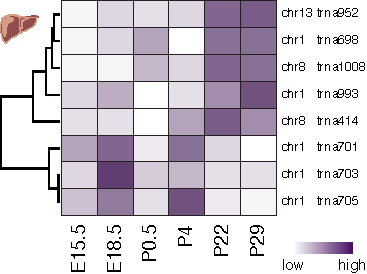
\includegraphics[width=\textwidth]{correlation-cag}
        \subcaption{\label{fig:compensation-a}Isoacceptor CAG \trna gene
            expression levels}
    \end{minipage}
    \hspace{0.05\textwidth}%
    \begin{minipage}{0.4\textwidth}
        \centering
        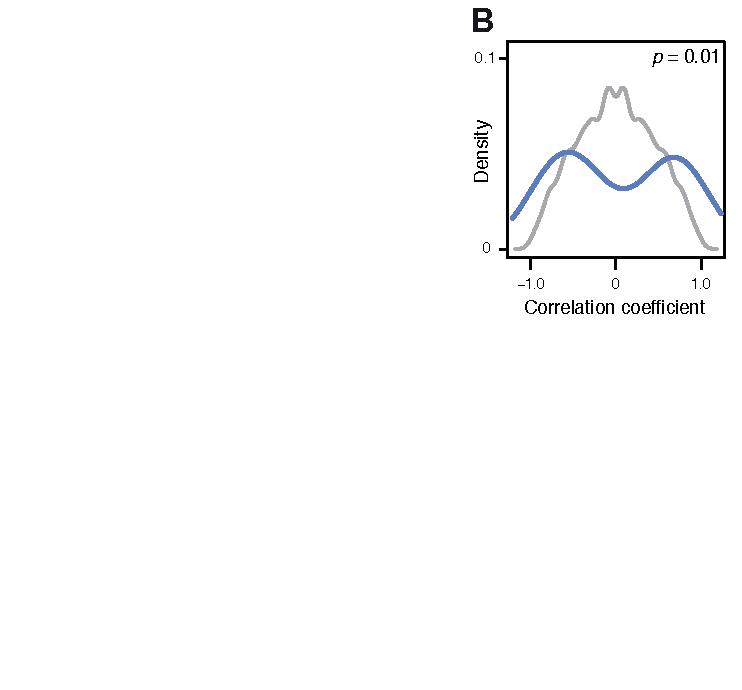
\includegraphics[width=\textwidth]{compensation-cag}
        \subcaption{\label{fig:compensation-b}Density curve of isoacceptor CAG
            \trna gene expression correlations}
    \end{minipage}
    \par
    \begin{minipage}{0.45\textwidth}
        \centering
        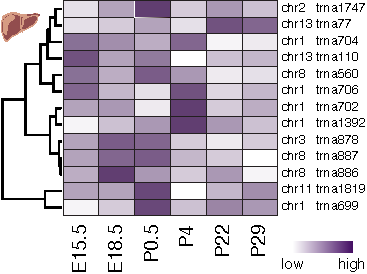
\includegraphics[width=\textwidth]{correlation-gcc}
        \subcaption{\label{fig:compensation-c}Isoacceptor GCC \trna gene
            expression levels}
    \end{minipage}
    \hspace{0.05\textwidth}%
    \begin{minipage}{0.4\textwidth}
        \centering
        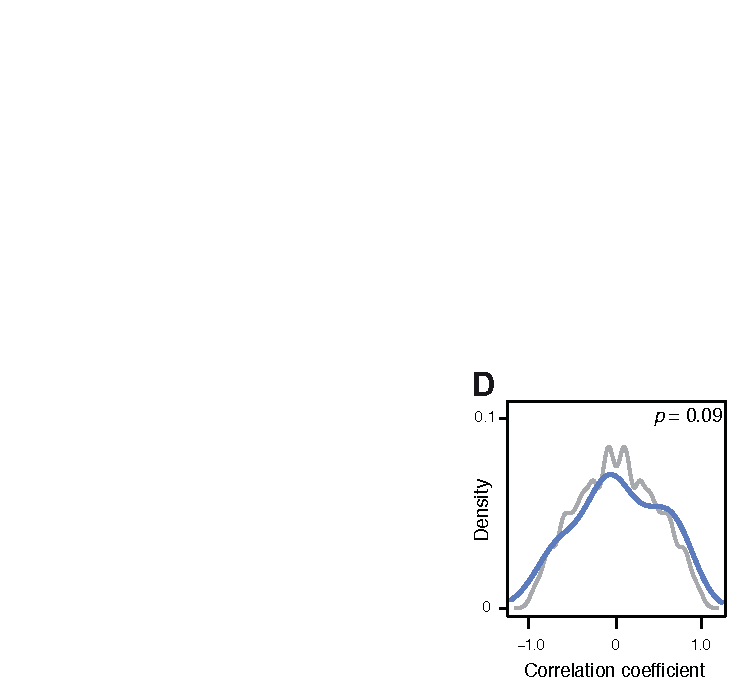
\includegraphics[width=\textwidth]{compensation-gcc}
        \subcaption{\label{fig:compensation-d}Density curve of isoacceptor GCC
            \trna gene expression correlations}
    \end{minipage}}
    {\trna gene expression is compensated at the anticodon isoacceptor level
    during mouse development.}
    {…}

\begin{table}[h!]
    \centering
    \begin{tabular}{@{}lS@{}}
        \toprule
        Isoacceptor & \multicolumn{1}{r@{}}{{\(p\)-value}}\\
        \midrule
        \anticodon{GUG} & 1.01E-25 \\
\anticodon{AGC} & 2.26E-12 \\
\anticodon{GCA} & 9.17E-11 \\
\anticodon{CCA} & 1.15E-10 \\
\anticodon{CUG} & 3.60E-09 \\
\anticodon{UGG} & 3.68E-07 \\
\anticodon{AAC} & 3.68E-07 \\
\anticodon{GUA} & 5.69E-06 \\
\anticodon{CAU} & 8.53E-06 \\
\anticodon{UUC} & 2.42E-05 \\
\anticodon{UGC} & 2.56E-05 \\
\anticodon{AGA} & 6.57E-05 \\
\anticodon{CUC} & 6.81E-05 \\
\anticodon{CAC} & 2.06E-04 \\
\anticodon{GUC} & 8.76E-04 \\
\anticodon{CAG} & 1.99E-02 \\
\anticodon{GUU} & 6.01E-02 \\
\anticodon{AGU} & 1.26E-01 \\
\anticodon{GCC} & 1.33E-01 \\
\anticodon{UUU} & 3.35E-01 \\
\anticodon{GCU} & 3.45E-01 \\
\anticodon{AAU} & 3.45E-01 \\
\anticodon{GAA} & 6.50E-01 \\
\anticodon{ACG} & 8.01E-01 \\
\anticodon{UCC} & 8.01E-01 \\
\anticodon{CUU} & 8.12E-01 \\
\anticodon{AGG} & 8.44E-01 \\

        \bottomrule
    \end{tabular}

    \tabcap{compensation}{Evidence against absence of compensation.}
    {The first column contains the \trna anticodon isoacceptor families. The
    second column the FDR-adjusted \(p\)-values of \(H_0\): there is no effect
    of the order of the stages on coordinated gene expression of \trna genes
    within an isoacceptor family.}
\end{table}
